\section{Przebieg rozgrywki (Bartosz Strzelecki, Bogna Lew)}\label{s:rozgrywka}
Gracz zaraz po rozpoczęciu rozgrywki znajduje się w małej wiosce (rys. \ref{fig:village}). Pierwszym
elementem przyciągającym uwagę gracza, jest postać o imieniu Amargein (rys. \ref{fig:npc}), która oferuje
nagrodę za pokonanie groźnego niedźwiedzia buszującego w pobliskim lesie. Użytkownik jednak
szybko się orientuje, że nie jest w stanie pokonać bestii w pojedynkę.

\begin{figure}[h]
\centering
\includegraphics[width=1\textwidth]{images/village}
\caption{Kadr z gry przedstawiający wioskę, w której gracz rozpoczyna rozgrywkę.}
\label{fig:village}
\end{figure}
\FloatBarrier

\begin{figure}[h]
\centering
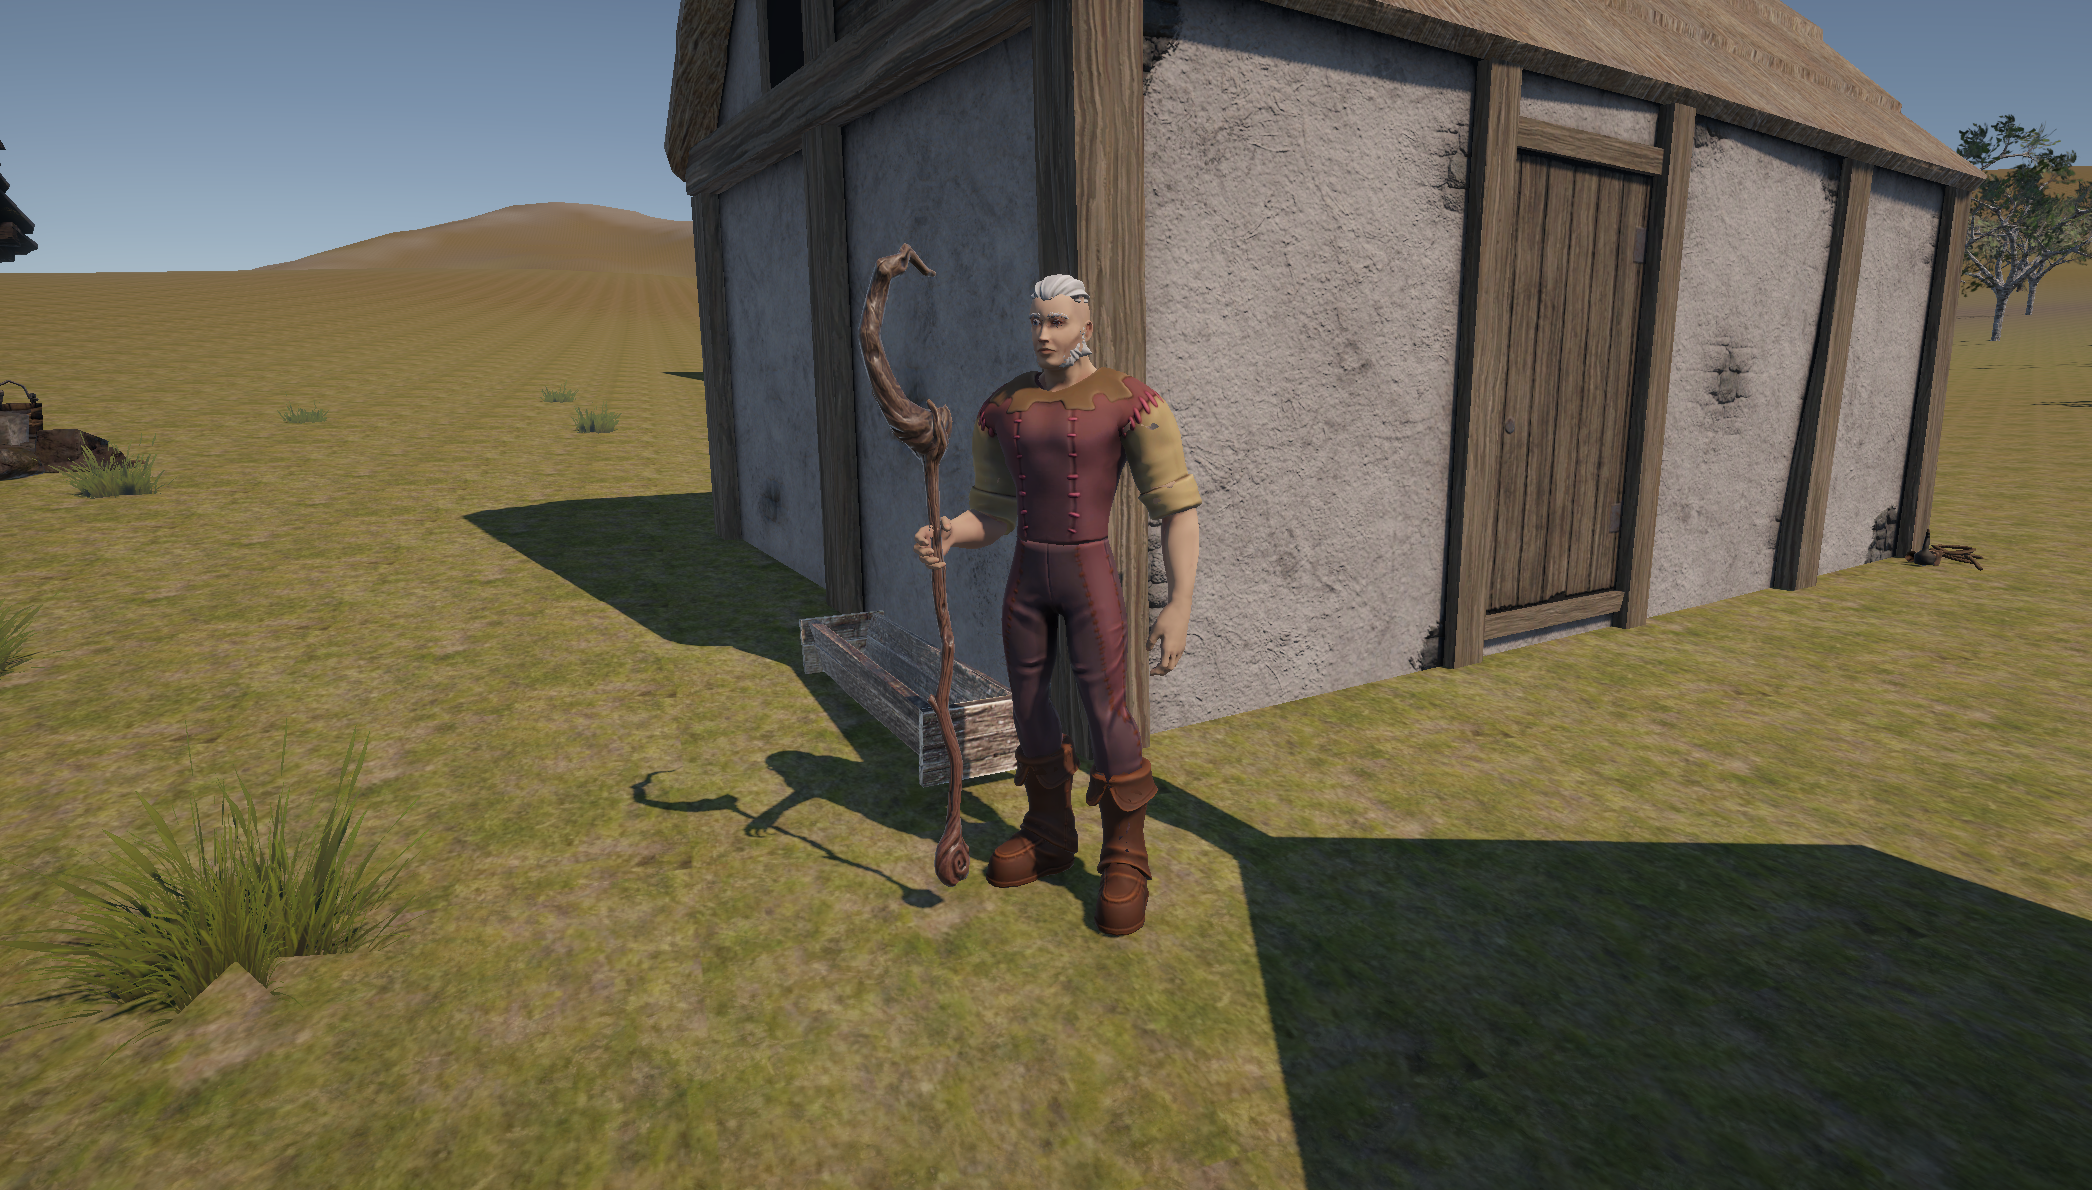
\includegraphics[width=1\textwidth]{images/npc1}
\caption{Kadr z gry przedstawiający postać niezależną zlecającą zadanie postaci gracza.}
\label{fig:npc}
\end{figure}
\FloatBarrier

Po głębszych poszukiwaniach gracz znajduje dwójkę najemników (rys. \ref{fig:mercs}), którzy byliby w stanie
wesprzeć główną postać za odpowiednią opłatą. Początkowo użytkownik nie może sobie
pozwolić na takie wydatki i jest zmuszony do znalezienia prostszego zadania
w celu zadbania o odpowiedni stan finansów.

\begin{figure}[h]
\centering
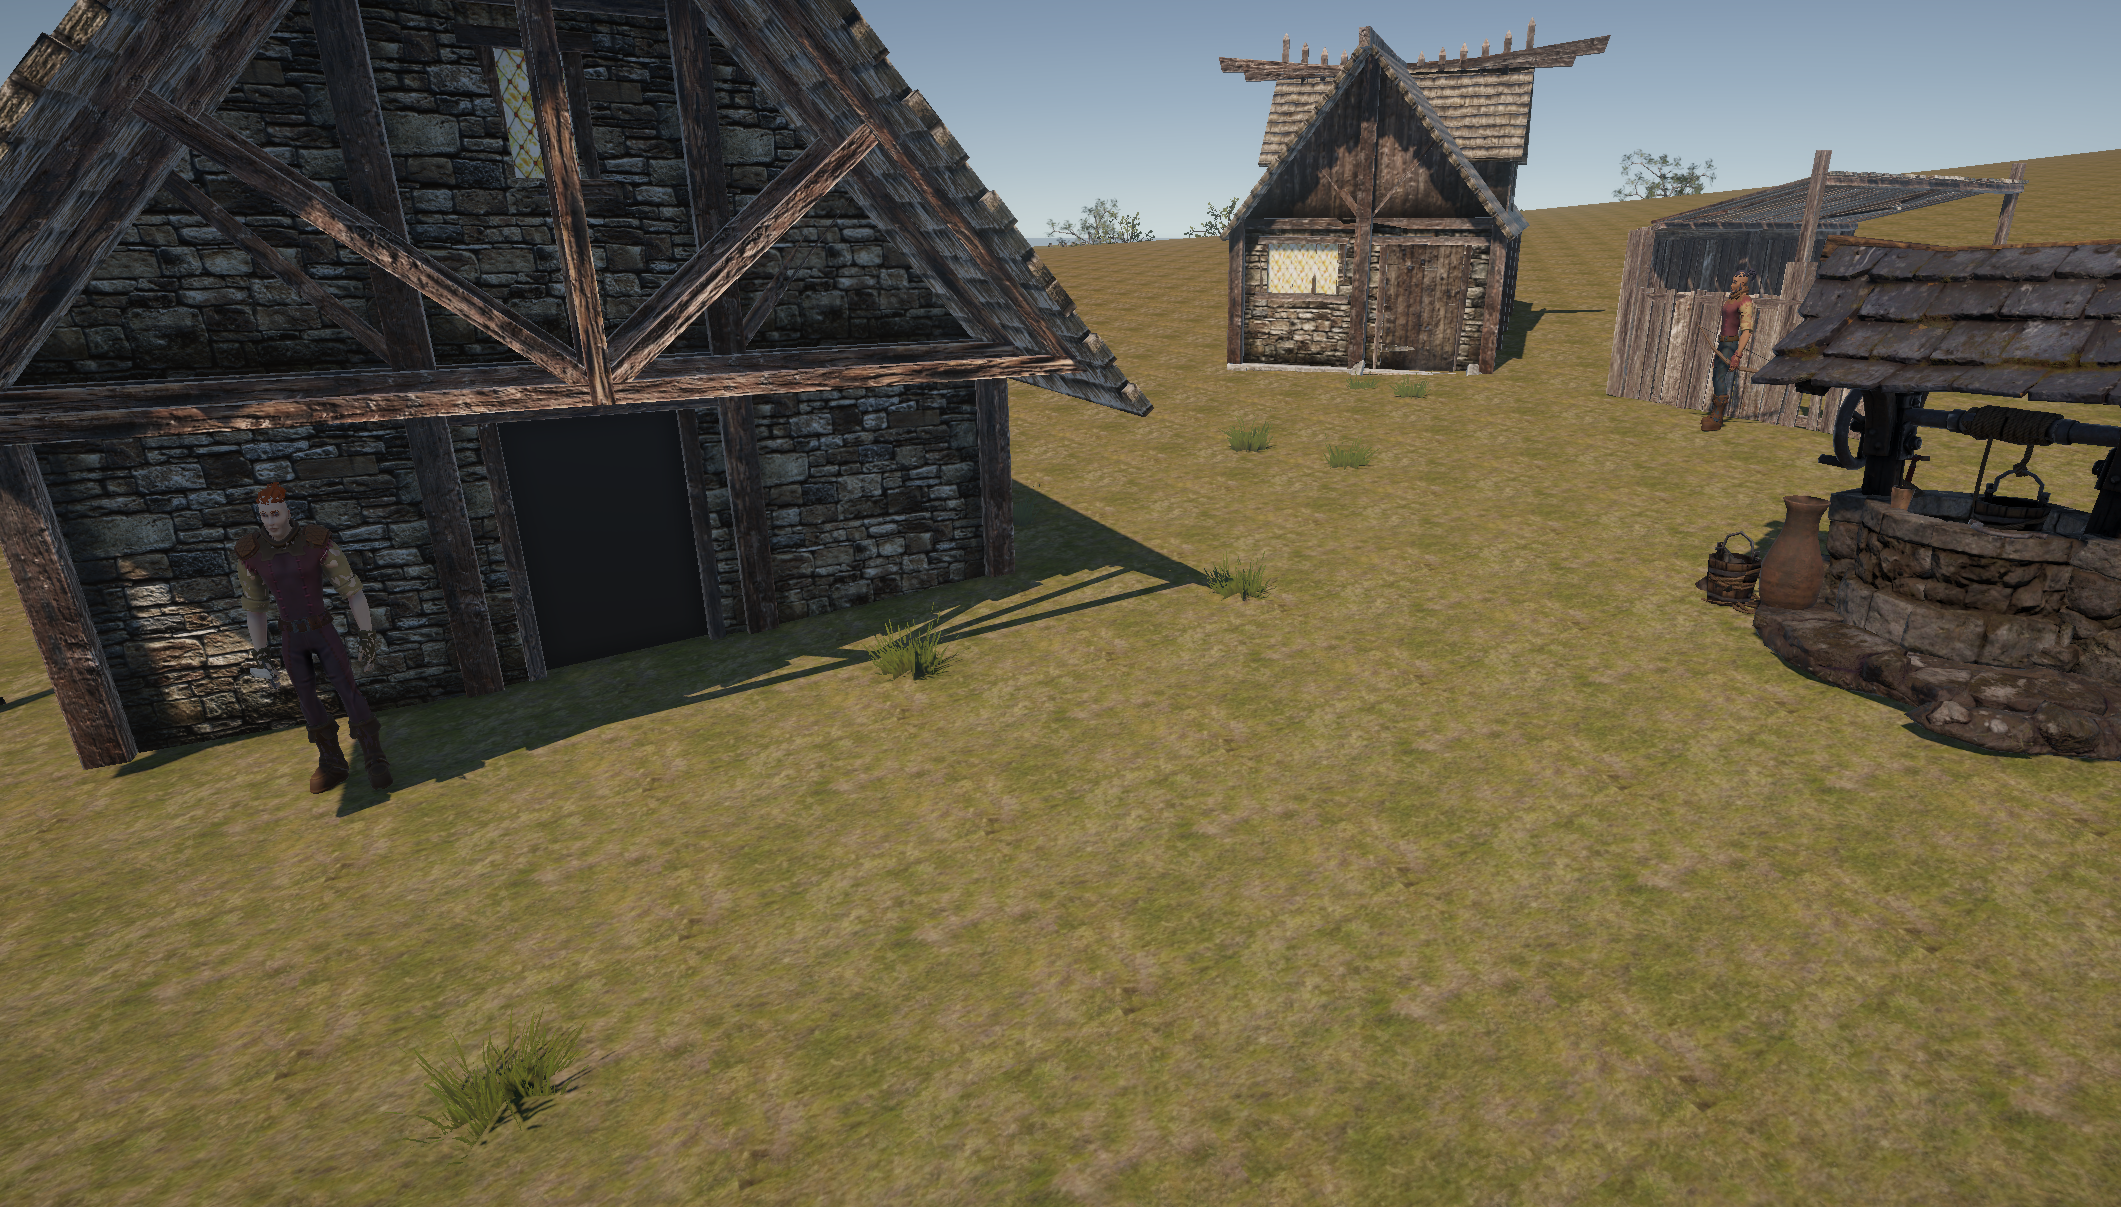
\includegraphics[width=0.8\textwidth]{images/mercs}
\caption{Kadr z gry przedstawiający możliwych do wynajęcia najemników.}
\label{fig:mercs}
\end{figure}
\FloatBarrier

Nieopodal wioski gracz dostrzega stojącego samotnie budowniczego. Po podejściu do niego, dowiaduje się, że nazywa się on
Rhodan i potrzebuje pomocy. Z jego opowieści wynika, że niedawno stracił cały swój dobytek w
pożarze i teraz nie ma gdzie mieszkać.

\begin{figure}[h!]
    \centering
    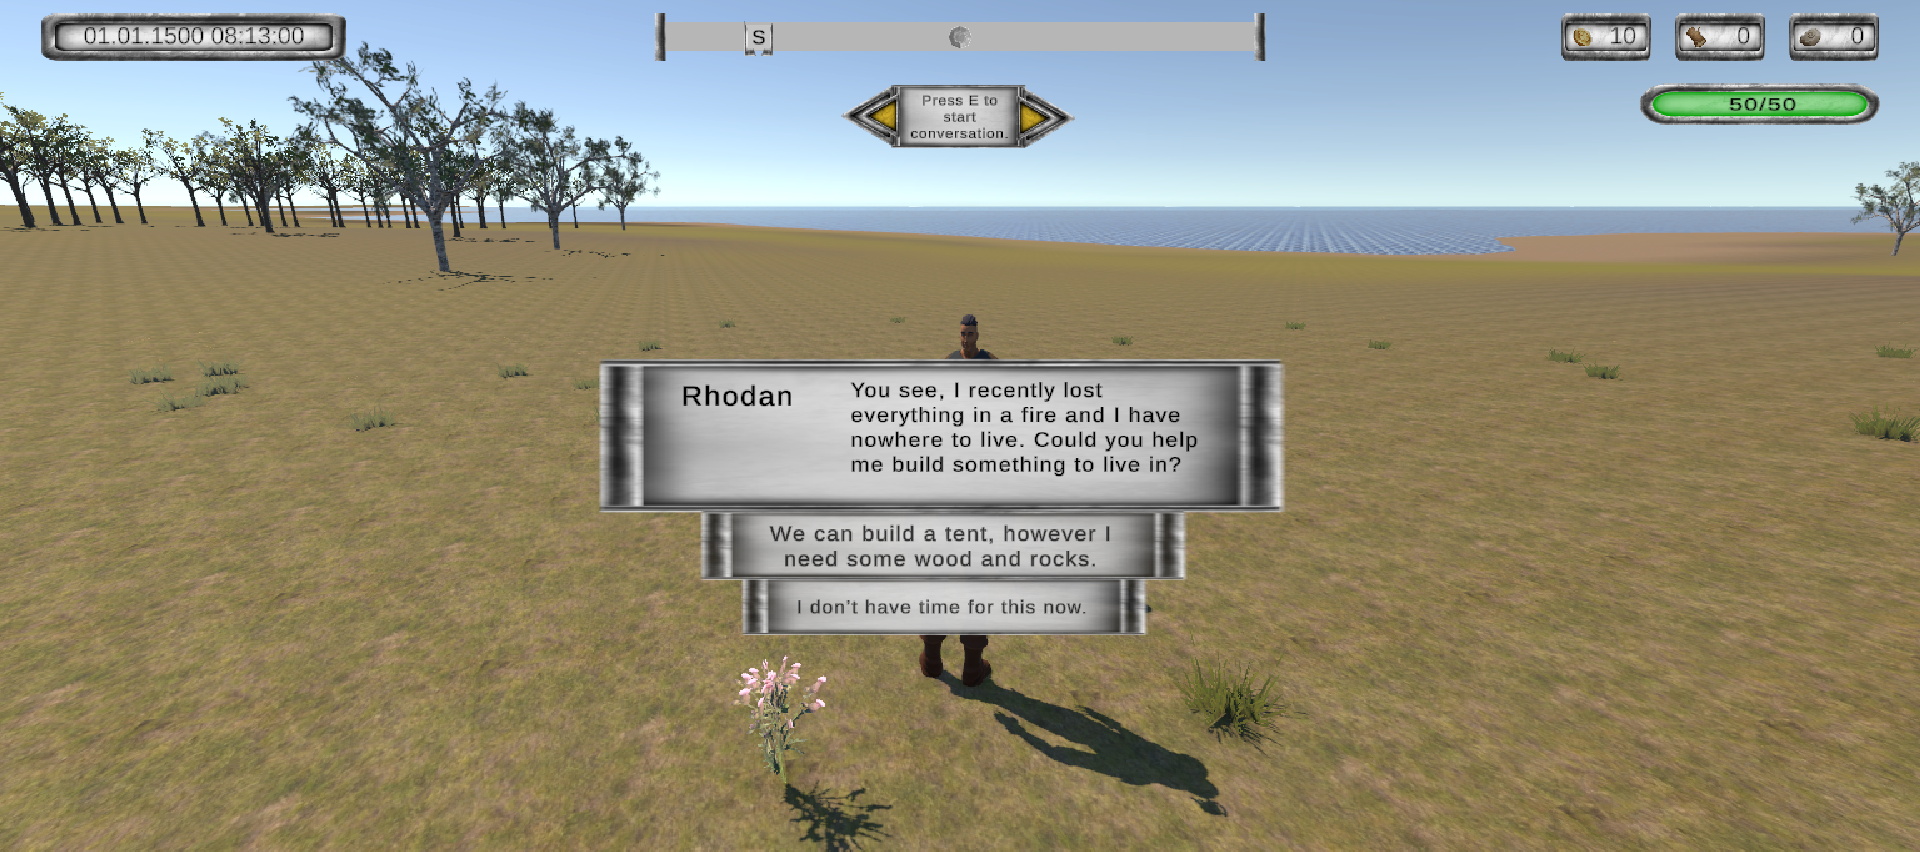
\includegraphics[width=1\textwidth]{images/rozgrywka/rhodan3.png}
    \caption{Kadr z dialogu z Rhodanem podczas którego opowiada swoją historię.}
\end{figure}
\FloatBarrier

Gracz proponuje mu wybudowanie namiotu, jednakże wymaga to zasobów, których nie posiada. Zapytawszy Rhodana gdzie mógłby
je zdobyć, dowiaduje się, że na zachodzie na skraju lasu leżą kłody oraz kamienie, które może spróbować zebrać. Zgodnie
z sugestią, gracz postanawia udać się w to miejsce, aby uzbierać wymagane surowce.

\begin{figure}[h!]
    \centering
    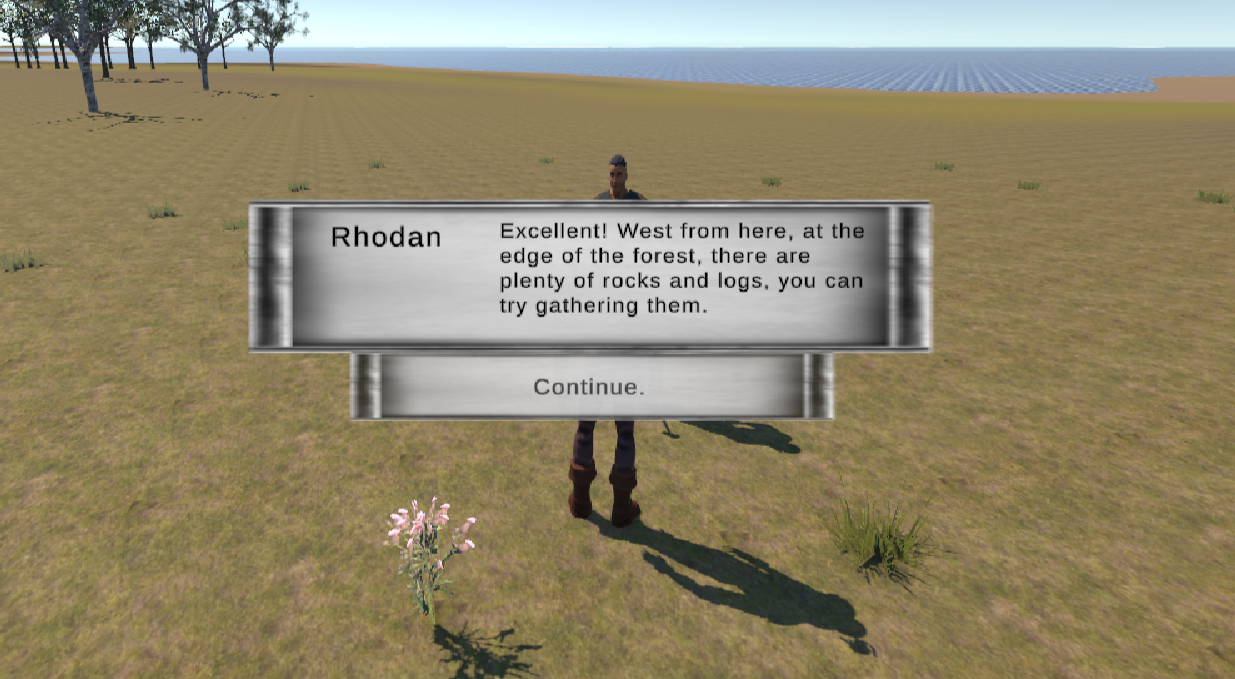
\includegraphics[width=1\textwidth]{images/rozgrywka/rhodan4.png}
    \caption{Kadr z dialogu z Rhodanem z wytycznymi odnośnie zbierania zasobów.}
\end{figure}
\FloatBarrier

Po zebraniu zasobów wraca porozmawiać z Rhodanem. Dowiaduje się od niego, że gdy mu wskaże odpowiednie do budowy namiotu
miejsce, to postać podejdzie i go wybuduje. Tak jak został poinstruowany, gracz wybiera miejsce, które nadawałoby się
pod budowę namiotu, a Rhodan podbiega i rozpoczyna budowę, wspomagając się młotkiem. Gdy mężczyzna skończył pracę gracz
odbiera swoją nagrodę.

\begin{figure}[h!]
    \centering
    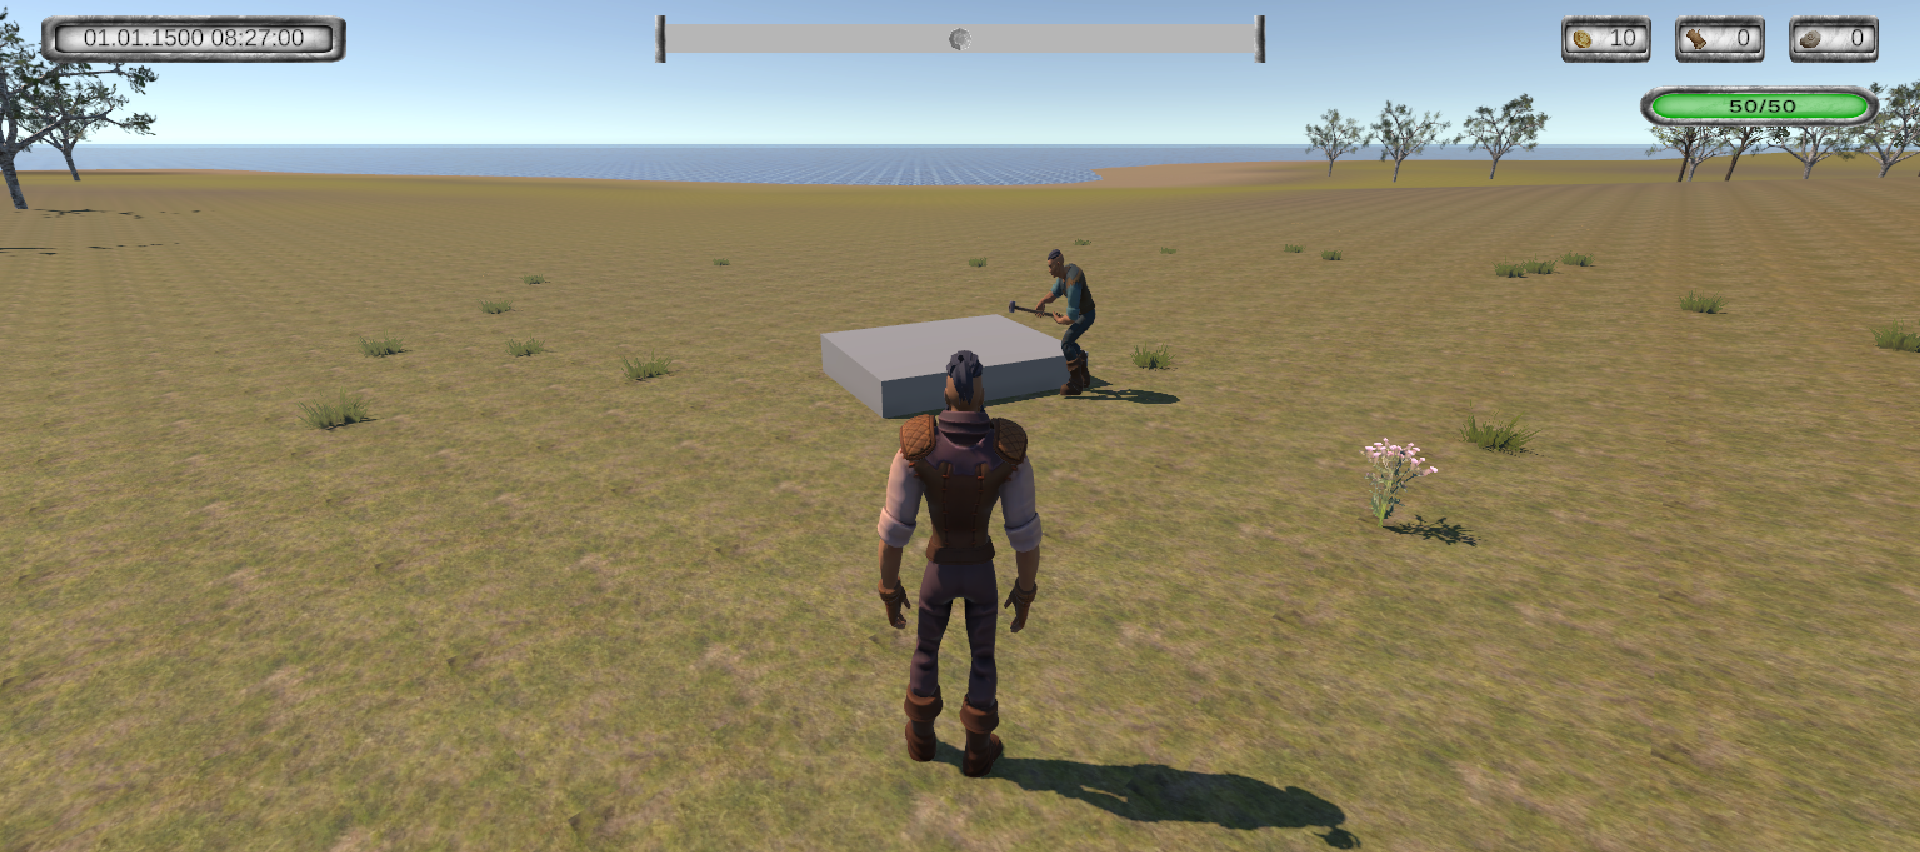
\includegraphics[width=1\textwidth]{images/rozgrywka/rhodan9.png}
    \caption{Kadr z gry, na którym widać budującego Rhodana.}
\end{figure}
\FloatBarrier

Po wykonaniu uprzedniego zadania gracz jest już w stanie wykupić pomoc dwóch okolicznych
najemników. Po rozmowie każdy z nich jest gotów zgodzić się na opłatę w wysokości 10 złotych monet.
Tak przygotowana drużyna gracza jest gotowa na wyruszenie na przygodę, by uratować
mieszkańców wioski od niedźwiedzia terroryzującego osadę.

Gracz, wykorzystując swoje zdolności nawigacji, udaje się na wschód i po krótkim czasie jest w stanie zidentyfikować zagrożenie.
Widząc swój cel, gracz wydaje rozkaz ataku. Wynajęte jednostki szybko uporały się z niedźwiedziem. Każda jednostka wykorzystywała
broń, z którą jest jak najbardziej biegła, czyli broń białą lub łuk.

\begin{figure}[h]
\centering
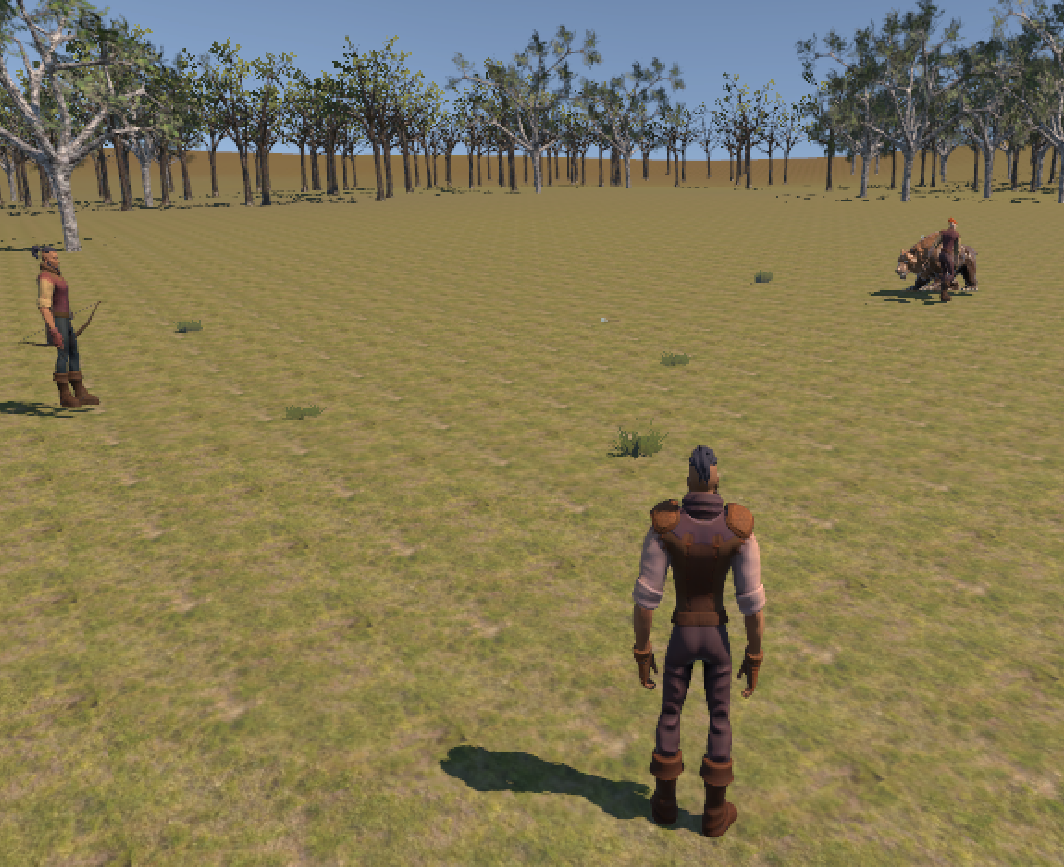
\includegraphics[width=1\textwidth]{images/fight}
\caption{Kadr z gry przedstawiający dwóch najemników toczących walkę z niedźwiedziem.}
\end{figure}
\FloatBarrier

Po powrocie do wioski gracz jest uznany za bohatera, który ocalił wszystkich mieszkańców i zostaje odpowiednio nagrodzony.

